% !TeX spellcheck = en_GB
%Introduction
%\begin{savequote}[50mm]
%If our brains were simple enough for us to understand them, we'd be so simple that we couldn't.
%\qauthor{Ian Stewart }%The Collapse of Chaos: Discovering Simplicity in a Complex World
%\end{savequote}

\section{Overview}

In the recent years, we are witnessing a constant growth in the usage of video streaming applications. Increasing of commonly used Live Streaming and Video-on-Demand (VOD) services, as well as the raising of new media applications involving video streams are gaining relevance and are attracting a wider audience. In this context, online gaming and video conferencing are highly popular, while 3D video formats enable support for eXtended Reality (XR), Virtual Reality (VR) and Augmented Reality (AR). Moreover, tailored streaming solutions are being employed to empower different vertical applications, e.g., Industrial Internet of Things (IIoT), medical imaging and automotive machine-vision, which can benefit from the advances in video streaming. Meanwhile, wireless and mobile devices are becoming the primary User Equipment (UE) for both content generation and consumption \cite{wolf2015news}.

It is evident that video streaming technologies are being used beyond traditional content playback as an alternative to television broadcasting. This means changes at different levels, from players and servers to media formats and delivery protocols, which also affect network traffic. 5G networks are expected to cope with the increasing total network traffic, mostly generated by media services, by means of higher network bandwidth and reduced latency. According to Cisco reports and forecasts, it is estimated that 5G connections will handle nearly three times more traffic than a current LTE connection by 2023 \cite{Cisco2020}. The estimation is still passive from being reviewed, as a larger usage of media applications than the expectation is being fuelled by the global COVID-19 pandemic. This pandemic is transforming users' habits to access the Internet \cite{Lutu2020, Feldmann2020} and media contents \cite{Favale2020, King2020}. The Broadband Commission for Sustainable Development, a joint initiative of the International Telecommunication Union (ITU) and the United Nations Educational, Scientific and Cultural Organization (UNESCO), is concerned about these trends and is implementing an Agenda for Action to push an emergency response to the pandemic, aiming at Internet access extension and boosting its capacity \cite{BroadbandCommission, ICTaffordability}.

All the mentioned factors are driving the evolution and the deployment of 5G networks and services. New network solutions are necessary to support high quality of service (QoS) for media applications, as a best-effort network approach to manage media traffic does not ensure the fulfilment of the requirements requested by the media service in terms of Key Performance Indicators (KPIs). Media services have constraints regarding packet delivery, e.g., on-time delivery or packet loss, which need to be addressed to guarantee a certain level of QoS. Therefore, lower QoS may result in lower user's quality perception, i.e., quality of experience (QoE). A pragmatic example of this QoE degradation are stalls or artifacts during video playback on player devices. Moreover, the heterogeneity of media-related use cases results in having different requirements depending on the specific media service, i.e., real-time communications from a security camera and VOD for entertainment have different requirements in terms of latency and throughput.

An essential system for streaming multimedia content is the Content Delivery Network (CDN). A CDN is the most common solution to increase the performance of online applications, including the video streaming ones. It consists in a geographically distributed hierarchical system to cache and deliver every type of contents, i.e., web objects (HTML web pages) or downloadable files (media files and documents). For video streaming purpose, a CDN provides the infrastructure to deliver Live or on-demand streams by fostering the efficiency and increasing the service coverage. The increasing number of internet users and the proliferation of video and rich media contents over the internet is boosting the demand for CDN solutions. The global CDN market is expected to grow at a rate of 14.1\% per year until 2025 \cite{CDNMarkets}.
The proliferation of CDNs is making their price to decrease, but the overall cost for the content provider (CP), which makes use of them to deliver its contents, is still increasing, as also the traffic volume from/to CDN is increasing \cite{Rayburn2020}.

Beyond CDNs, more advanced solutions based on Software Defined Network (SDN) \cite{kreutz2014software} and Network Function Virtualization (NFV) \cite{Han2015} technologies are being investigated to boost media services.
SDN is a network management approach to enable a centralized and programmable way to configure and monitor the network and its performance. It separates the control from the data plane such that the network administrator can configure the network resources in an easy way. The control layer includes a SDN controller provided with an Application Programming Interface (API) that allows to fill and updates the forwarding tables of the network infrastructure (data plane or forwarding plane). The data plane processes and forward the data packets based on the instructions coming from the control plane. 
NFV is instead a network architecture concept that uses virtualization technologies to deploy and operate an infrastructure totally independent of hardware. In other words, it decouples network functions from the commercial off-the-shelf (COTS) hardware where they are deployed and run. Network functions, called Virtual Network Functions (VNFs), are deployed and connected to create a complete network service (NS) on top of a virtualized infrastructure.
Definitively, SDN and NFV represent complementary solutions. NFV virtualizes the network infrastructure (Core, Edge and Access Networks) built on top of data centers, while SDN centralizes network control and manages the forwarding rules between data centers. The combination of them allows to have networks and services that are operated and managed by software systems running on top of COTS hardware.
It is important to note that 5G is pushing the employment of SDN and NFV to manage end-to-end connections and to provide them with the demanded network resources. Within the 5G umbrella, Multi-access Edge Computing (MEC) \cite{etsi2019} also covers an important role to guarantee end-to-end performance. MEC is a new architectural concept to provide virtualized capabilities at Network Edge. MEC platform consists in an NFV-compliant data center to deploy and run VNFs close to the Radio Access Network (RAN). Additionally, it also provisions a specific API to access Radio Network Information (RNI) \cite{etsigsmec012}. A RNI service (RNIS) oversees the collection of RNI which can be consumed by VNFs running at MEC host.

In video streaming context, VNFs can be employed at any level of the end-to-end communication (Core, Edge and Access Networks) to empower network capabilities when generating, delivering and/or consuming video streaming traffic in an optimized and cost-effective manner \cite{Jahromi2018, Dieye2018}. VNFs enable flexible operations with several benefits. Firstly, VNF-based networks monitor objective operational parameters, such as throughput or latency, representative for QoS of the streaming dataflows, which have a direct influence on user's satisfaction.
However, QoS metrics do not perfectly map on user experience, as user perceived quality is highly subjective. Additionally, QoE which compiles subjective evaluation elements, including rewards for playback quality and smoothness, and penalties for image freezes and unstable or low quality \cite{Kim2010, Alreshoodi2013}, needs to be considered, too.
Secondly, the CP has more control to shape the network traffic and allocate resources since business rules for VNF deployment and life-cycle management could be established. These rules allow to adjust network resources and business costs trade-offs \cite{Hernandez2015}, so they are highly relevant.
%Last, as the volume, complexity and real-time nature of streaming traffic has an evident impact on energy consumption of the network and devices managing the content, an optimized streaming delivery through VNFs should also consider the energy efficiency.

In general, selecting the right performance metrics to optimize the video streaming is not trivial. There is not a unique metric to evaluate the goodness of a particular media solution, as multiple viewpoints coexist. Network Operator (NO) is interested in providing a QoS according to the Service Level Agreement (SLA) contracted by the CP or the user, while keeping Operational Expenditure (OPEX) under a target threshold.
CP has to guarantee the best QoE to the users, while aiming in business costs reduction.
Finally, the users are mostly interested in having as higher and steadier QoE as possible.
%Finally, energy consumption metrics are meant to become more crucial, even for media services, as energy efficiency is a worldwide critical challenge.
In any case, it is clear that performance assessment and network monitoring are important sources of information that can be exploited for the design of performance-driven VNFs for media services. Thus, information from performance metrics and network monitoring allows to optimize the network service.

\section{Motivation}

As described in the previous section, network services depend on the characteristics and performance provided by the underlying network. Monitoring the network and assessing performance metrics are essential for improving the services.
%It is no more possible to consider network capabilities enhancement and media service improvement as separate optimization problems.
Considering network capabilities enhancement and media service improvement as separate optimization problems is not a good option as they are intrinsically related.
5G ships new parameters and technologies which make the difference in enhancing both the network itself and the services running on it. Media services are deployed as Virtual Network Functions (VNFs), which run on top of an NFV Infrastructure (NFVI) and are interconnected through SDN rules.
Moreover, the benefits gained from deploying a network-aware media service are evident, as the media service can react to variable network conditions. Combining innovative media services with KPIs improvements introduced by 5G, it is possible to achieve more reliable and flexible networks and services, where the exploitation of performance metrics and network information is essential for performance-driven optimization.

HTTP Adaptive Streaming (HAS) \cite{Seufert2014} is a video streaming technology that was natively designed to exploit measurements performed on the network by the media player. Video content is encoded at different representation bitrates and resolutions and the player is in charge of selecting the one that fits with the network measurements and its internal state (playback buffer size or window of time buffered for the playback). The different representations are also split in segments of fixed duration (between 2 and 10 seconds), enabling switching operations between representations each time a new segment needs to be downloaded.
HAS implementations, such as HTTP Live Streaming (HLS) \cite{hls2017} and Dynamic Adaptive Streaming over HTTP (MPEG-DASH) \cite{sodagar2011mpeg}, can be furtherly improved, as they present two main limitations. First, uncoordinated operations between players sharing the network assets may cause unfairness, as the resources could not be equally distributed. Second, HAS intrinsically has high latency as a segment cannot be sent until fully generated. The theoretical minimum latency is the segment duration which makes impossible to achieve real-time communications.
This thesis is oriented to improve video streaming services by exploiting the information coming from the performance metrics and network traffic monitoring and analysis. Moreover, it aims to provide solutions to overcome the current limitations of HAS.

\begin{figure}[htp]
	\centering
	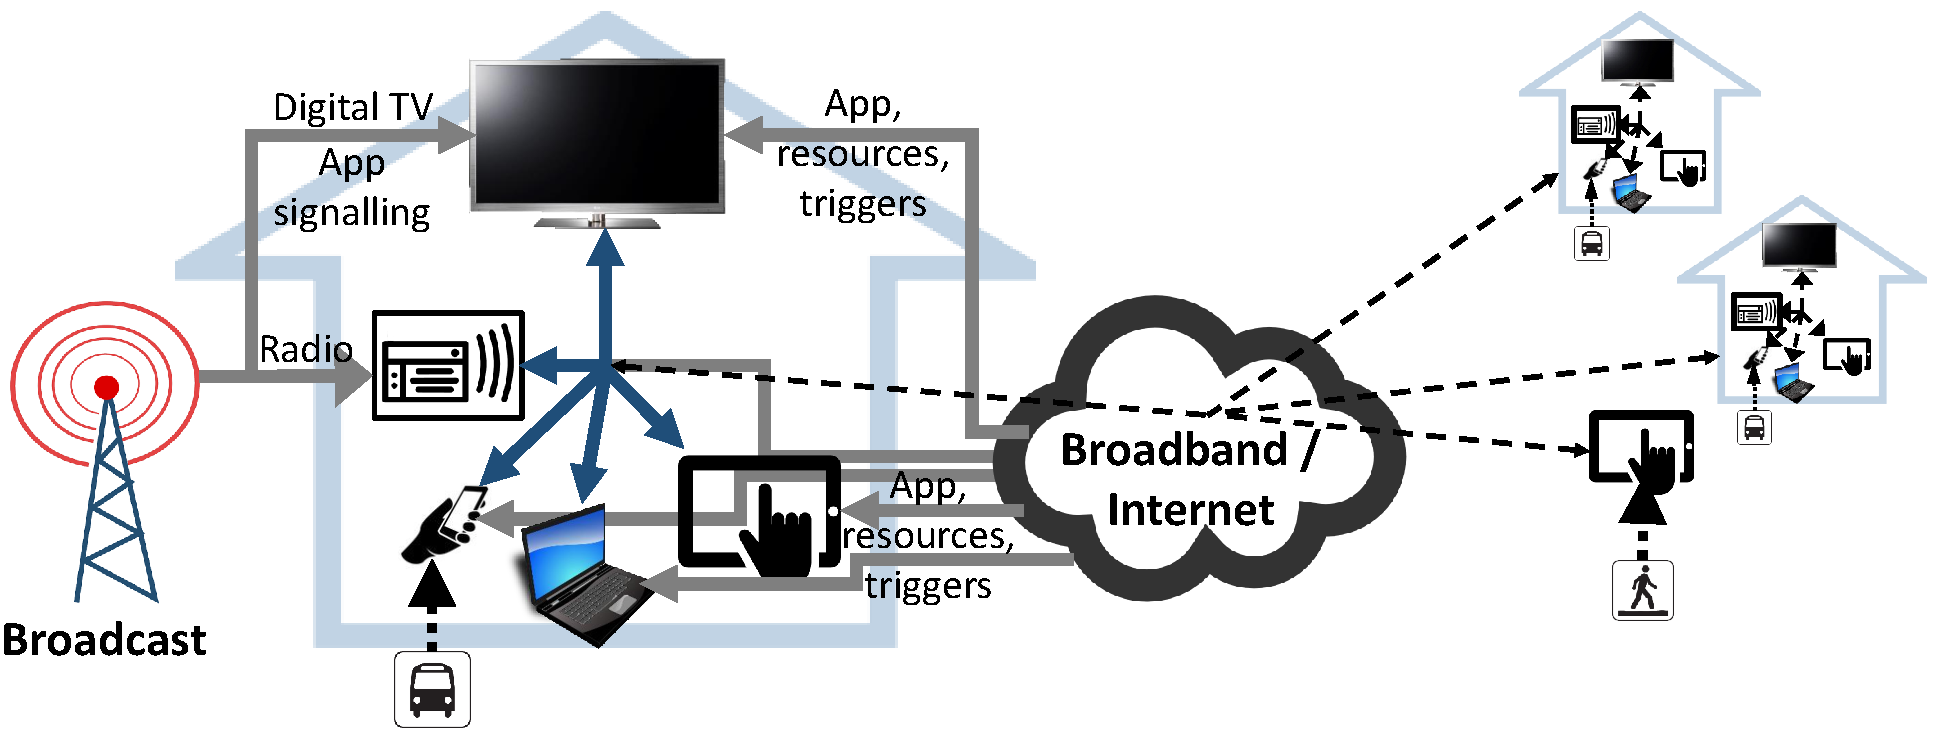
\includegraphics[width=1\textwidth]{ecosystem.pdf}
	\caption{Overview of a video streaming communication and involved stakeholders and/or agents.}
	\label{fig:ecosystem}
\end{figure}

Figure \ref{fig:ecosystem} includes all the stakeholders and/or agents coming into play in a common video streaming communication schema.
First, the origin server, managed by the CP, generates the content by performing two main operations. It encodes the video content through standard codecs, e.g., H264 \cite{wiegand2003} or HEVC \cite{sullivan2012overview}. Then, it packages it in a streaming format/protocol that is later sent to the CDNs. Here, the encoded and packaged content is stored and distributed to the end users. When considering HAS technologies, an additional manifest file is generated and stored in a media server and it is accessed by the media player to know the available representations and the CDNs where media segments are cached. 
Optionally, the manifest stored at the media server can be periodically updated, as declared in the standard, to provide the player with updated information on the available representations and the CDN. Thus, it enables to serve a different manifest to each request and influence the player's behavior in selecting the CDN from which downloading the content, as well as selecting the representation of each segment.
Finally, mobility trends are pushing solutions that move from legacy streaming between remote servers (origin server or CDN) and media players to more complex ones that include MEC-based services in the middle of the end-to-end streaming process.
HAS enables individual optimization of the QoE performed by each player. It is not an optimal solution, as it may cause unfairness in terms of QoE among end users.
The awareness of RNI at the MEC allows to assess network QoS and estimate user's QoE. It enables the possibility to take actions that enforce QoS/QoE and fairness among the players.
MEC-enabled solutions include the possibility to locally cache HAS video segments and, again, to modify the manifest in a coordinated way with the remote media server and the CDNs.

This research work is focused on some major changes in the video streaming context.
\textbf{First}, the knowledge of network information can be exploited to encode the content at the appropriate video bitrate and resolution and select the media container format.
\textbf{Second}, when delivering the content, network metrics can be monitored and analyzed to forecast the behavior of the network and take proactive actions to optimize the delivery.
\textbf{Third}, the introduction of MEC within the 5G umbrella enables the development and deployment of services close to the RAN, which empower the delivery through network and video analytics.
In the following paragraphs, the motivation for each of them is explained.

\textbf{First}, when preparing the video content to be delivered, two main operations are required: compressing the content through standard video codecs, e.g., H.264 or HEVC, and packaging it in media container formats, e.g., MPEG-4 Part 14 (commonly called MP4). Encoding and packaging the content influence user's QoE, which plays a significant role when dealing with media services, as a satisfactory QoE may help to retain the user from leaving the media service. Human Visual System (HVS) has been widely studied for years when developing the actual video codecs in order to increase the compression rate, while keeping the same quality of the image \cite{torres2012video}, and further improvements are expected by the next generation ones. Moreover, Per-Title Encoding \cite{PerTitle2015} strategy also includes the complexity of the video content itself in the equation. Per-Title Encoding targets to select the encoding bitrate for the chosen codec that best fits with the visual complexity. Thus, it aims to present a paramount view experience.
%QoE scores are unchanged, but the usage of computational and memory resources is being optimized. Moreover, business costs to sustain the encoding process are reduced, as resources are being saved.

In any case, video codec development and Per-Title strategy are only focused on the user's QoE and does not consider the possibility to exploit network information to optimize the encoding process. If the network is not able to provide sufficient throughput to cope with encoded bitrate, stalls and video artifacts are experienced at the media player which affects the QoE. HAS aims to reduce the number of stalls by allowing the player to select the video representation, among the available ones, that fits with the experienced network performance. Here, uncoordinated operations and unfairness between players, as well as HAS intrinsic high latency, are still major issues to be addressed.

To overcome such limitations and to provide bitrate adaptation according to network conditions, two different options are envisioned:
\begin{itemize}
	\item Introducing bitrate adaptation on top of streaming protocols designed for real-time communications.
	\item Enabling the possibility to send partially generated HAS segment to the client, such that the content is sent to the player with minimum delay after the encoding operation. This solution is the key of Low Latency Common Media Application Format (LL CMAF) \cite{hughes2017information}, also called Chunked CMAF.
\end{itemize}
The former solution also enables coordinated delivery as the bitrate is chosen by the origin server which is generating the content, but it lacks scalability as unicast streams are generated independently for each video session. The latter solution keeps the advantages provided by HTTP protocol, such as the possibility to cross Network Address Translation (NAT) systems and firewall devices, and end user device heterogeneity, as every device supports HTTP.

\textbf{Second}, in-network caching is a mechanism to improve the performance when accessing online contents and, in particular, media streaming ones. It aims to prevent negative effects on the QoS/QoE caused by network impairments. In this context, a CDN is the popular solution to cache and deliver video streams. Furthermore, major CPs also moved to multi-CDN strategies to provide a more reliable service while streaming their contents \cite{adhikari2012, adhikari2012-2}. In a multi-CDN environment, several strategies on how selecting the best performing CDN are applicable by the CP, but they are typically limited to a selection at the startup, keeping the same CDN along all the streaming session \cite{adhikari2015}.

Enabling the capability to switch between alternative CDNs, when the streaming sessions are ongoing, opens to lots of possibilities for optimization.
%Optimizing the usage of CDN resources can reduce the business costs for the CP.
Thus, multi-CDN strategies can be designed to optimize CDNs utilization and reduce the resultant OPEX for the CP. Among these strategies, proactive ones can exploit forecasts to perform actions which cope with a predicted increased demand and/or prevent the effects of predicted network failures.

\textbf{Third}, 5G includes MEC \cite{etsi2019} as key pillar to increase the performance of network applications. MEC is a new network architecture concept that enables computing capability close to the RAN to run algorithms and/or services that empower specific applications. RNIS integrated into MEC platform allows the deployed services to access RNI report and exploit it. Thus, it fosters the design and development of use cases and/or vertical sector-specific solutions that exploit the favorable location near the RAN and the context of the network \cite{Tan2018, Martin2019}.

In any case, the information provided by the RNIS consists in a set of objective metrics, i.e., RNIS assesses only information related to QoS. Designing and developing QoE models for their deployment at the MEC represents a step forward. When considering media streaming applications, a QoE model can infer RNI/QoS metrics to estimate the QoE experienced by the end users. Being able to access both QoS and QoE information at the MEC increases the interest of CPs to design MEC-empowered algorithms and/or services that take actions to improve their media service performance. MEC solutions should address two main objectives. First, a MEC-enabled media solution should maximize both the QoS and QoE, while trying to reduce the network traffic volume. Thus, the objective is to optimize the trade-off between QoS/QoE and business costs for network assets. Second, the assessment of the QoE of each individual player should foster solutions that improve the fair utilization of the network resources. Consequently, fairness in viewing experience can be increased through fair sharing the network assets. This produce similar playback at media players.

Eventually, to fully understand the scope of our research and its challenges, the following list summarizes the considered contextual factors regarding the demographic trends in media consumption habits of users together with technological alternatives and business models:

\begin{enumerate}
	
	\item Multimedia consumption is gradually shifting from traditional TV to Over-the-top (OTT) media services where the CP streams media contents via the Internet. Utilization of both mobile devices, i.e., smartphones and tablets, and connected TVs, including flat-panel TVs, set-top boxes and gaming consoles, will grow during the next few years. By 2023, the consumer share of the total devices will be 74\%, with business claiming the remaining 26\% \cite{Cisco2020}.
	
	\item Video streaming is heavily dominating the traffic over the Internet, as the demand of higher and higher quality video contents is increasing the consumption on network resources. It is fueled by improved cameras with stunning picture quality \cite{saad2015} and the breakthroughs in display technology \cite{kathirgamanathan2015electroluminescent}. By 2023, 66\% of connected flat-panel TV sets will be 4K \cite{Cisco2020} and 47\% of all devices and connections will be video capable \cite{Cisco2020-2}.
	
	\item Increasing video resolutions, such as 4K and 8K, and the rise of new video formats, such XR, VR and AR, is pushing the development of new compression techniques and codecs. Improved video codecs for 2D images are being released in the recent years \cite{chen2018overview, sidaty2019compression}, while 3D compression is finally being standardized \cite{schwarz2018emerging}.
	
	\item International consortia, such as the European Telecommunications Standards Institute (ETSI) and the International Telecommunication Union (ITU), are driving the digital transformation of the networks. Softwarization and virtualization are changing the economics of the networks and pushing NOs to move from proprietary and specific hardware to virtualized software platforms through the abstraction of the execution environment \cite{Hernandez2015}.
	
	\item ETSI proposes the deployment of edge services at MEC infrastructures and includes several use cases related to media streaming \cite{etsigsmec002}. MEC platform can host diverse edge services, which exploit RNI to get a wider view of the local conditions to enhance media streaming service \cite{Tan2018, Martin2019}. Moreover, the capillarity of MEC concept allows to run edge services whose nature is distributed.
	
	\item When managing the networks, a Service Level Agreement (SLA) aims to enforce network capabilities for a specific service. Modern network services require different levels of guaranteed bandwidth, latency and priority over other traffic. Thus, avoiding SLA violations is becoming more and more important to guarantee required performance over time \cite{badshah2020performance}.
	
\end{enumerate}

All these mentioned trends are reinforced and aligned with the experience acquired by participating in several national and European projects, such as 5G \hbox{Euskadi} (\url{https://5g-euskadi.com/}), Open-VERSO (\url{https://www.openverso.org/en/}) and Fed4Fire+ (\url{https://www.fed4fire.eu/}). These projects involve first level telecommunication operators, such as Orange (\url{https://www.orange.es/}) and Euskaltel (\url{https://www.euskaltel.com/}), technology providers, such as ZTE (\url{https://www.zte.com.cn/global/}), universities, such as University of \hbox{Thessaly} (\url{https://nitlab.inf.uth.gr/NITlab/nitos}), and research institutes, such as Vicomtech (\url{https://www.vicomtech.org/en}), Gradiant (\url{https://www.gradiant.org/en/}) and i2Cat (\url{https://i2cat.net/}).

\section{Hypothesis}

The working hypothesis is constructed as a statement of the following expectations:

\begin{enumerate}
	\item Encoding operations at the origin server are improved if compression schemes and encoding strategies make use of the information provided by both the video content and the network status.
	\item Utilization of network assets is optimized by leveraging information achieved by monitoring network and media players' behavior.
	\item Distributed nature of MEC concept enables the deployment of services focused on supporting enhanced media session management and performance.
%	\begin{enumerate}[label=(a)]
%		\item 
%		\item 
%	\end{enumerate}
\end{enumerate}

These mentioned expectations involve different stakeholders and/or agents in the media streaming chain shown in Figure \ref{fig:ecosystem}:

\begin{itemize}

	\item \textbf{Content Provider}
	\begin{itemize}
		\item It manages both origin and media servers, even they do not necessarily belong to it, as they could be deployed in a third-party cloud platform.
		\item It aims to reduce business costs for the exploitation of network assets, including cloud and MEC platforms and CDN resources.
	\end{itemize}
	
	\item \textbf{Content Delivery Network (CDN) vendor}
	\begin{itemize}
		\item It provides CDN infrastructure to store and deliver media contents.
		\item It grants an SLA with CPs that has to respect by avoiding/reducing violations.
	\end{itemize}

	\item \textbf{Network Operator (NO)}
	\begin{itemize}
		\item It provides network resources (Core, Edge and RAN) to stream the content from the CDNs to the end users.
		\item More than one NO's network could be crossed when streaming a content, i.e., multi-domain networks.
		\item MEC hosts and services are deployed and managed close to NO's RAN infrastructure.
		\item It grants SLAs with both CPs and end users that has to respect by avoiding/reducing violations.
	\end{itemize}

	\item \textbf{End User}
	\begin{itemize}
		\item It is subscribed to CP's media service.
		\item It is connected to the network thanks to its network provider (Network Operator).
		\item It is receiving the media stream on its player device and watching it.
		\item It aims to have the highest possible QoE.
	\end{itemize}

\end{itemize}	

%\hl{Add hypothesis figure.}

%\begin{figure}[htp]
%	\centering
%	\subfloat[]{\includegraphics[width=1\textwidth]{hypothesis_service-cropped.pdf}%
%		\label{fig:hypothesis_service}}
%	\hfil
%	\subfloat[]{\includegraphics[width=1\textwidth]{hypothesis_user-cropped.pdf}%
%		\label{fig:hypothesis_user}}
%	\hfil
%	\subfloat[]{\includegraphics[width=1\textwidth]{hypothesis_network-cropped.pdf}%
%		\label{fig:hypothesis_network}}
%	\hfil
%	\caption[Diagram of the hypothesis for the perception of \textbf{(a)} the \textit{media service}, \textbf{(b)} the \textit{users} and \textbf{(c)} the \textit{mobile network operator} for an enhanced experience.]{Diagram of the hypothesis of the perception of \textbf{(a)} the media service, \textbf{(b)} the users and  \textbf{(c)} the mobile network operator for an enhanced experience.}
%	\label{fig:hypothesis}
%\end{figure}


\section{Objectives}

The main objective of this work is to improve QoS and QoE of media streaming, while reducing CP's business costs. Performance of video streaming services are evolved by means of advanced encoding solutions and new 5G network architecture and paradigms. Furthermore, the main objective is decomposed into more specific objectives:

\begin{enumerate}
	\item Enabling advanced encoding and packaging strategies with the aim of exploiting the information acquired from the network to improve the encoding operations with focus on media streaming QoS and user's QoE.
	\item Empower media delivery by using Machine Learning (ML) algorithms to allow the CP to reduce business costs, while guaranteeing a sufficient level of QoS.
	\item Integrate MEC platform and develop services that enforce media streaming sessions and boost the user's QoE.
\end{enumerate}

\begin{figure}[htp]
	\centering
	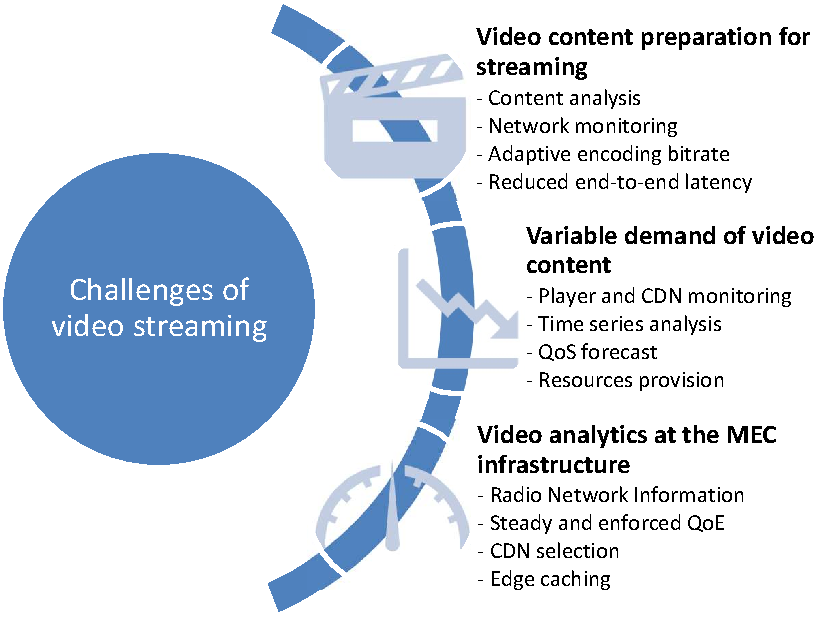
\includegraphics[width=0.8\textwidth]{thesis-challenges.pdf}
	\caption{Main challenges to be addressed in order to achieve the objectives of this Ph.D. thesis.}
	\label{fig:objectives}
\end{figure}


To achieve these objectives, it is necessary to address and provide solutions to overcome the three main challenges of video streaming (see Figure \ref{fig:objectives}):

\begin{enumerate}
	\item \textbf{Video content preparation for streaming:}
	%it is no more possible to consider network and media service QoS and user's QoE as separate optimization problems.
	considering network QoS enhancement and user's QoE improvement as separate optimization problems is not a good option as they are intrinsically related.
	The origin and media servers should be provided with the knowledge acquired from the network. Network-aware servers can take actions to balance network QoS and user's QoE.	
	\item \textbf{Variable demand of video contents:} number of users and their demanded contents are varying. It causes complex network dynamics, where the traffic depends on the demanded contents and the representation bitrate chosen to stream them at any moment. Increasing or decreasing the employed network assets depending on the demand means efficiently managing the resources and finding a trade-off that ensures a steady and consistent user's QoE and reduces CP's business costs.
	\item \textbf{Video analytics at the MEC infrastructure:} the 5G MEC architecture exploits network performance metrics at the RAN to estimate user's QoE. Therefore, the possibility to boost user's media streaming session is envisioned by influencing the caching and CDN selection strategies and minimizing the impact of network faults or issues on the QoE.
\end{enumerate}

\section{Contributions}

The main contribution of this Ph.D. research is founded on the advances in video streaming technologies to provide enhanced performance of media services. Various metrics are defined to consider performance from different point of view, including business costs, network capacity and user's satisfaction. These advances, based on standard protocols and technologies, enable network-aware and performance-driven video streaming solutions which operate on dynamic and flexible networks.

More specifically, the main contribution can be translated into specific outcomes. Figure \ref{fig:contributions} illustrates the three specific contributions of the research in a wider context to address content generation and delivery, and management of the network and its resources.

\begin{figure}[htp]
	\centering
	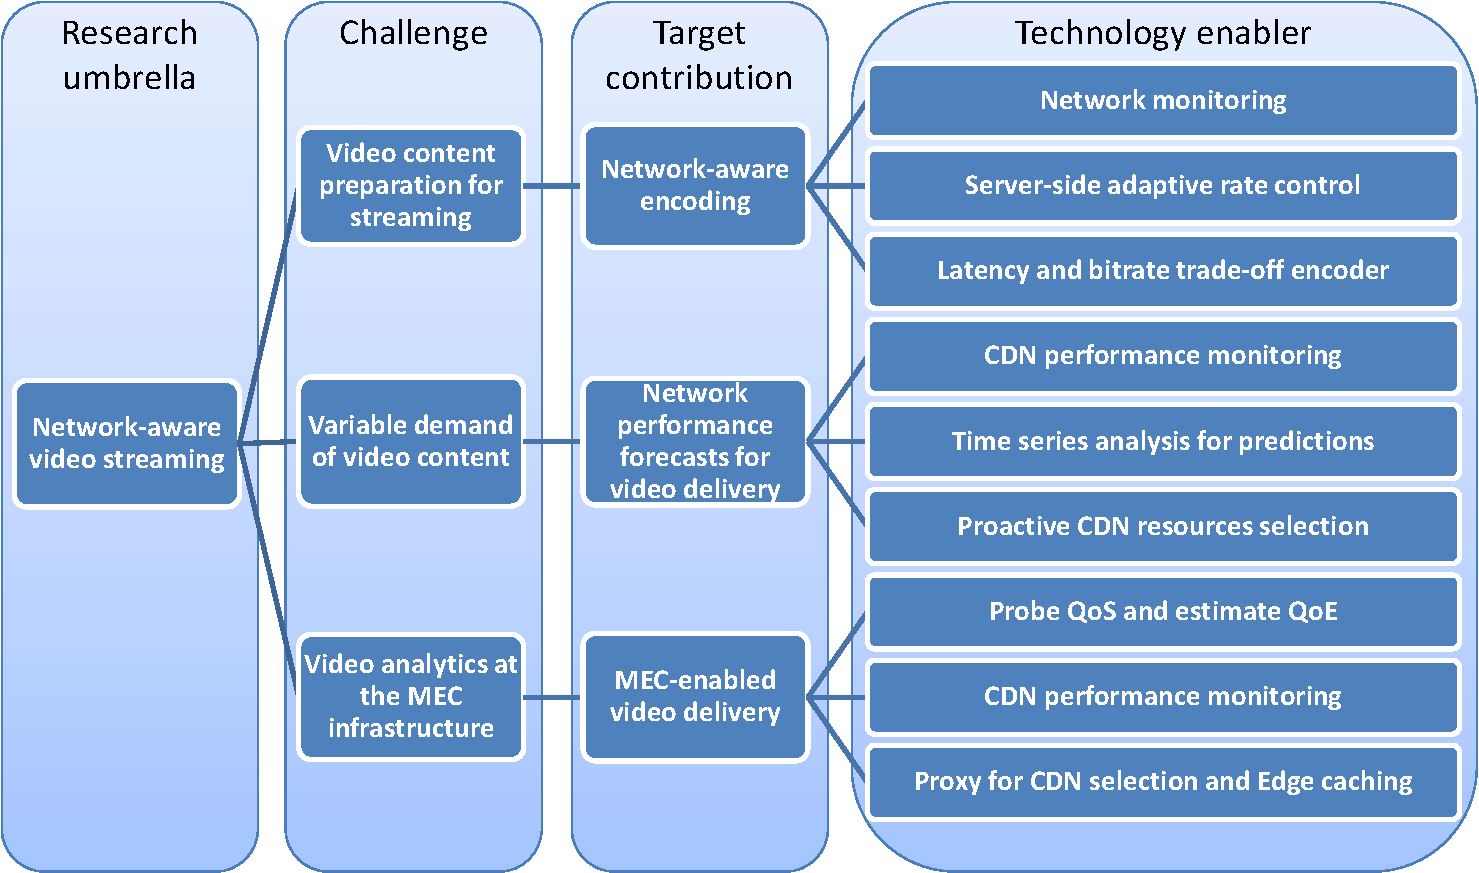
\includegraphics[width=1\textwidth]{contributions.pdf}
	\caption{Diagram of the contributions of the research.}
	\label{fig:contributions}
\end{figure}

%\subsubsection{Contribution 1: Network-aware video encoding}
\textbf{\underline{Contribution 1: Network-aware video encoding}}
\label{contribution:1}

Optimizing video encoding and packaging strategy has effects on user's QoE, which plays a significant role when dealing with media services, as a satisfactory QoE may retain the user from leaving the media service. Studies on HVS \cite{torres2012video} and Per-Title Encoding \cite{PerTitle2015} are leading to analyse the video image complexity in order to apply custom encoding settings for different classes of video contents (e.g., action movie, sport, security camera, etc.), which optimize the exploitation of video processing resources, while enhancing user's QoE.

Including network information and application context (VOD or real-time communications) represents a further step. Selection of video encoding bitrate and streaming format/protocol should be chosen depending on the application context and network information. In this sense, this thesis has designed and implemented two different solutions that exploit such information.

First, on top of SRT protocol, an Adaptive Rate Control is developed to demonstrate the applicability of network information at the origin server. It enables a coordinated delivery as the encoding bitrate is chosen by the origin server once for all the connected media players. Second, a solution which exploits the wide support of end devices for playing HAS streams, such as MPEG-DASH and HLS, studies LL CMAF to deliver Live Streaming and evaluates the trade-off between latency and QoE.

Publications related to Contribution 1:
\begin{itemize}
	\item \textit{R. Viola, \'A. Mart\'in, J. F. Mogoll\'on, A. Gabilondo, J. Morgade and M. Zorrilla, "Adaptive Rate Control for Live streaming using SRT protocol," 2020 IEEE International Symposium on Broadband Multimedia Systems and Broadcasting (BMSB), pp. 1-6, 2020, doi: 10.1109/BMSB49480.2020.9379708}, in Section \ref{chap:BMSB2020}.
	\item \textit{R. Viola, A. Gabilondo, \'A. Mart\'in, J. F. Mogoll\'on and M. Zorrilla, "QoE-based enhancements of Chunked CMAF over low latency video streams," 2019 IEEE International Symposium on Broadband Multimedia Systems and Broadcasting (BMSB), pp. 1-6, 2019, doi: 10.1109/BMSB47279.2019.8971894}, in Section \ref{chap:BMSB2019}.
\end{itemize}

%\subsubsection{Contribution 2: Network performance forecasts for video delivery}
\textbf{\underline{Contribution 2: Network performance forecasts for video delivery}}
\label{contribution:2}

CDN is a common solution to provide caching capabilities with worldwide coverage, as it is a geographically distributed hierarchical system that cache and deliver online contents and, in particular, media streaming ones. Thus, the usage of CDN aims to prevent negative effects on the QoS/QoE caused by network impairments. CPs make extensive use of CDNs, also including strategies that employ several CDNs at the same time \cite{adhikari2012, adhikari2012-2}. Then, it implies the definition of more complex CDN selection mechanisms. In any case, the typical solution consists in CDN selection at the media player session startup, keeping this selection along all the streaming session \cite{adhikari2015}.

In this context, the ability to switch between different CDNs, when streaming sessions are in progress, represents an interesting approach. It allows to optimize the employed CDN resources by reducing their usage to the effective necessity. As the number of players connected to a CDN increases, migrating some players to another CDN helps maintain QoS and QoE scores. In contrast, when the number of players decreases, migrating all players to a single CDN reduces the CDN resources used.

This thesis designed a multi-CDN strategy that optimizes CDNs utilization and reduce the resultant business costs for it. The solution is empowered with a trained Artificial Neural Network (ANN) model that forecasts network performance to perform proactive actions which cope with a predicted increased demand and/or prevent the effects of predicted network failures.

Publications related to Contribution 2:
\begin{itemize}
	\item \textit{R. Viola, \'A. Mart\'in, J. Morgade, S. Masneri, M. Zorrilla, P. Angueira and J. Montalb\'an, "Predictive CDN selection for video delivery based on LSTM network performance forecasts and cost-effective trade-offs," IEEE Transactions on Broadcasting, vol. 67, no.1, pp. 145-158, 2020, doi: 10.1109/TBC.2020.3031724}, in Section \ref{chap:IEEETBC2020}.
\end{itemize}


%\subsubsection{Contribution 3: MEC-enabled video delivery}
\textbf{\underline{Contribution 3: MEC-enabled video delivery}}
\label{contribution:3}

MEC architecture \cite{etsi2019} has been designed to increase the performance of 5G networks by enabling computing capability closer to the users, in the RAN segment of the network. It allows to run algorithms and/or services that empower specific applications. To further improve MEC services, a RNI Service (RNIS) deployed at the MEC provides a specific API to access RAN information or RNI \cite{etsigsmec012}. The information provided by the RNIS consists in a set of objective metrics that is possible to infer in order to understand the end device and player's behavior. Knowledge of the behavior allows to that take actions to improve the media session performance.

Such information fosters the design and development of use case-specific solutions, including media steaming ones \cite{Tan2018, Martin2019}, as specified by ETSI \cite{etsigsmec002}. The favorable location near the RAN and the provided RNI represent important assets to be exploited for the design of the MEC service. In this sense, this thesis has designed and implemented two different solutions that infer and exploit information acquired at the MEC platform.

First, a MEC service is designed to run on top of a Wi-Fi access point \cite{etsigsmecwifi}. It allows to collect player's objective metrics, such as bitrate and resolution of the video representation, switching operations between representations, number of stalls and their duration, and infer them to estimate the user's QoE with high accuracy. Second, a MEC proxy is developed to exploit information at the RAN by enabling local caching and CDN selection at the edge network.

Publications related to Contribution 3:
\begin{itemize}
	\item \textit{R. Viola, M. Zorrilla, P. Angueira and J. Montalb\'an, "Multi-access Edge Computing video analytics of ITU-T P.1203 Quality of Experience for streaming monitoring in dense client cells," submitted to Multimedia Tools and Applications (March 25, 2021)}, in Section \ref{chap:MTAP2020}.
	\item \textit{R. Viola, \'A. Mart\'in, M. Zorrilla and J. Montalb\'an, "MEC Proxy for efficient cache and reliable multi-CDN video distribution," 2018 IEEE International Symposium on Broadband Multimedia Systems and Broadcasting (BMSB), pp. 1-7, 2018, doi: 10.1109/BMSB.2018.8436904}, in Section \ref{chap:BMSB2018}.
\end{itemize}

\subsection{Document structure}

This thesis has been structured as follows. Part \ref{sec:Part1} presents an introduction to the research scope, focusing on the motivation for the research, the hypothesis, the objectives and the contributions of the Ph.D. work. 

Part \ref{sec:Part2} overviews literature related to network functions for media streaming applications, including media encoding services and delivery solutions.

In Part \ref{sec:Part3}, the research results are described in three chapters:

\begin{itemize}
	\item Chapter \ref{chap:network-aware} describes the contributions to create video encoding and packaging solutions that exploit information acquired from the network and the application context (\textit{Contribution 1}). The goal is to tune the video processing operations in order to find the appropriate trade-off between latency and QoE when considering Live streaming applications.
	\item Chapter \ref{chap:predictive} describes the contributions to create video delivery strategies that exploit network performance forecasts in a multi-CDN context (\textit{Contribution 2}). The goal is to guarantee the required QoS for the media streaming application while reducing the business costs.
	\item Chapter \ref{chap:MEC} describes the contributions to create MEC services that estimate QoE scores and take actions to improve the streaming sessions (\textit{Contribution 3}). The goal is to infer RAN information to increase user's QoE by enabling local caching and CDN selection at the edge network.
\end{itemize}

In Part \ref{sec:Part4}, the conclusions of the research can be found, including a discussion that enables future work.

Part \ref{sec:appendix} provides an appendix, including other publications of the author, the resume, and a list of the acronyms employed throughout the document.

Finally, Part \ref{sec:bibliography} contains the bibliography.
